%!TEX root = mainfile.tex

\subsection{Calculations on Magnification} % (fold)
\label{sub:calculations_on_magnification}
	The following calculations were carried out in order to quantify the number of extra objects one would expect to see with a lens. A magnification factor $\mu$ is chosen which corresponds to a change in AB magnitude given by
	\begin{align}
		AB_\text{change} &= -2.5\log_{10}(\mu)
	\end{align}
	The fraction of the Einstein radius within which a source will be magnified by at least the value of $\mu$ is given to good approximation by\cite{Lens_mass_estimate}
	\begin{align}
		x_E &= \frac{\mu}{\mu -1}
	\end{align}
	Using the velocity dispersion of the cluster $\sigma$ and the angular diameter distances to the lens $D_L$ and source $D_S$ respectively, the following expression is also found to yield the Einstein angle,
	\begin{align}
		\theta_E &= \frac{4\pi G}{c^2}\frac{D_S-D_L}{D_S}
	\end{align}
	Using the Einstein angle in units of arcseconds, the area in degrees within which a certain magnification is exceeded is given by
	\begin{align}
		A &= \frac{\pi(x_E \theta_E)^2}{3600^2}
	\end{align}
	This area is calculated for source redshifts 1--15 and lens redshifts 0.1--1. Using results from the program written by the predictions subgroup which gives a value for the number of galaxies per square degree, the area calculated above is multiplied by each value, giving a number of sources magnified at each redshift and magnitude. If the area, $A$, is found to be larger than the field of view of the telescope being used, then $A$ is replaced by the field of view of the telescope as objects magnified outside of the field of view will not be observed. To find the number of extra galaxies seen with a lens between certain redshifts, one can sum the sources magnified enough to be seen in the redshift range of interest. For example, for a magnification of 10, sources as dim as magnitude 34.1 can be seen with JWST (without the lens, JWST would be limited to magnitude 31.6). One would sum for example redshifts 10--12 for magnitudes 31.6--34.1 to find the additional number of galaxies seen in this range.

	The magnification factors considered for these calculations are 15, 10, 5, 2.5 and 1.5 which enable telescopes to see magnitudes of 2.94, 2.5, 1.75, 1 and 0.44 deeper respectively. Selecting a lens at a redshift of 0.6 as an example, Table~\ref{tab:areas_table} shows the area magnified by a given factor for a range of source redshifts.
	\begin{table}[htbp]
		\begin{center}
			\begin{tabular}{c|c|c|c|c|c}
				Source $z$ 	&$\mu=1.5$	&$\mu=2.5$	&$\mu=5$	&$\mu=10$	&$\mu=15$ \\
				\hline \hline
			10	&\num{1.08e-3} 	&\num{3.33e-4} 	&\num{1.87e-4} 	&\num{1.48e-4} 	&\num{1.38e-4} \\
			11	&\num{1.09e-3} 	&\num{3.37e-4} 	&\num{1.90e-4} 	&\num{1.50e-4} 	&\num{1.39e-4} \\
			12	&\num{1.10e-3} 	&\num{3.41e-4} 	&\num{1.92e-4} 	&\num{1.51e-4} 	&\num{1.41e-4} \\
			13	&\num{1.11e-3} 	&\num{3.44e-4} 	&\num{1.93e-4} 	&\num{1.53e-4} 	&\num{1.42e-4} \\
			14	&\num{1.12e-3} 	&\num{3.46e-4} 	&\num{1.95e-4} 	&\num{1.54e-4} 	&\num{1.43e-4} \\
			15	&\num{1.13e-3} 	&\num{3.49e-4} 	&\num{1.96e-4} 	&\num{1.55e-4} 	&\num{1.44e-4}
			\end{tabular}
		\end{center}
		\caption[areas table]{Area within which the magnification factor is greater than certain values. These areas have been calculated using a lens redshift of 0.6 and a velocity dispersion of \SI{1000}{\kilo\metre\per\second}.\label{tab:areas_table}}
	\end{table}

	These areas correspond to the following numbers of extra sources observed at redshifts 10--15 for a cluster with velocity dispersion \SI{1000}{\kilo\metre\per\second} including any source now magnitude 31.6 or brighter.
	\begin{table}[htbp]
		\begin{center}
			\begin{tabular}{c|c|c|c|c|c}
				Source $z$ 	&$1.5>\mu$	&$1.5>\mu>2.5$	&$10>\mu>5$	&$15>\mu>10$	&$\mu>15$ \\
				\hline \hline
				10--12 		&4.19 		&2.97 			&2.33 		&1.42 			&25.2 \\
				12--15 		&1.21 		&1.04 			&1.00 		&0.70 			&13.2
			\end{tabular}
		\end{center}
		\caption[source numbers table]{Number of objects magnified by each factor, calculated from the areas in Table~\ref{tab:areas_table} and the predictions group's program.\label{tab:source_numbers_table}}
	\end{table}

	From Table~\ref{tab:source_numbers_table}, the highest number of extra sources observed have been magnified by a factor greater than 15. This is unsurprising, since at greater magnifications, the deepest sources will be observed, and the number density of galaxies is predicted to increase rapidly at dimmer magnitudes. Furthermore, the area within this smallest circle is larger than the differences between the intermediate areas so more sources will be seen here. In the mid regions, the source count is lower however once the magnification is as low as 2.5, the number begins to increase again, since the area within which such small magnifications can occur become very large. Figure~\ref{fig:distribution_of_magnification1} shows the distribution of redshifts of the magnified objects.
	\begin{figure}[htbp]
    	\begin{minipage}[c]{0.5\linewidth}
			\centering
				\begingroup\endlinechar=-1
					\resizebox{\textwidth}{!}{%
						% GNUPLOT: LaTeX picture with Postscript
\begingroup
  \makeatletter
  \providecommand\color[2][]{%
    \GenericError{(gnuplot) \space\space\space\@spaces}{%
      Package color not loaded in conjunction with
      terminal option `colourtext'%
    }{See the gnuplot documentation for explanation.%
    }{Either use 'blacktext' in gnuplot or load the package
      color.sty in LaTeX.}%
    \renewcommand\color[2][]{}%
  }%
  \providecommand\includegraphics[2][]{%
    \GenericError{(gnuplot) \space\space\space\@spaces}{%
      Package graphicx or graphics not loaded%
    }{See the gnuplot documentation for explanation.%
    }{The gnuplot epslatex terminal needs graphicx.sty or graphics.sty.}%
    \renewcommand\includegraphics[2][]{}%
  }%
  \providecommand\rotatebox[2]{#2}%
  \@ifundefined{ifGPcolor}{%
    \newif\ifGPcolor
    \GPcolortrue
  }{}%
  \@ifundefined{ifGPblacktext}{%
    \newif\ifGPblacktext
    \GPblacktexttrue
  }{}%
  % define a \g@addto@macro without @ in the name:
  \let\gplgaddtomacro\g@addto@macro
  % define empty templates for all commands taking text:
  \gdef\gplbacktext{}%
  \gdef\gplfronttext{}%
  \makeatother
  \ifGPblacktext
    % no textcolor at all
    \def\colorrgb#1{}%
    \def\colorgray#1{}%
  \else
    % gray or color?
    \ifGPcolor
      \def\colorrgb#1{\color[rgb]{#1}}%
      \def\colorgray#1{\color[gray]{#1}}%
      \expandafter\def\csname LTw\endcsname{\color{white}}%
      \expandafter\def\csname LTb\endcsname{\color{black}}%
      \expandafter\def\csname LTa\endcsname{\color{black}}%
      \expandafter\def\csname LT0\endcsname{\color[rgb]{1,0,0}}%
      \expandafter\def\csname LT1\endcsname{\color[rgb]{0,1,0}}%
      \expandafter\def\csname LT2\endcsname{\color[rgb]{0,0,1}}%
      \expandafter\def\csname LT3\endcsname{\color[rgb]{1,0,1}}%
      \expandafter\def\csname LT4\endcsname{\color[rgb]{0,1,1}}%
      \expandafter\def\csname LT5\endcsname{\color[rgb]{1,1,0}}%
      \expandafter\def\csname LT6\endcsname{\color[rgb]{0,0,0}}%
      \expandafter\def\csname LT7\endcsname{\color[rgb]{1,0.3,0}}%
      \expandafter\def\csname LT8\endcsname{\color[rgb]{0.5,0.5,0.5}}%
    \else
      % gray
      \def\colorrgb#1{\color{black}}%
      \def\colorgray#1{\color[gray]{#1}}%
      \expandafter\def\csname LTw\endcsname{\color{white}}%
      \expandafter\def\csname LTb\endcsname{\color{black}}%
      \expandafter\def\csname LTa\endcsname{\color{black}}%
      \expandafter\def\csname LT0\endcsname{\color{black}}%
      \expandafter\def\csname LT1\endcsname{\color{black}}%
      \expandafter\def\csname LT2\endcsname{\color{black}}%
      \expandafter\def\csname LT3\endcsname{\color{black}}%
      \expandafter\def\csname LT4\endcsname{\color{black}}%
      \expandafter\def\csname LT5\endcsname{\color{black}}%
      \expandafter\def\csname LT6\endcsname{\color{black}}%
      \expandafter\def\csname LT7\endcsname{\color{black}}%
      \expandafter\def\csname LT8\endcsname{\color{black}}%
    \fi
  \fi
  \setlength{\unitlength}{0.0500bp}%
  \begin{picture}(7200.00,4320.00)%
    \gplgaddtomacro\gplbacktext{%
      \put(543,595){\makebox(0,0)[r]{\strut{} 0}}%
      \put(543,986){\makebox(0,0)[r]{\strut{} 1}}%
      \put(543,1377){\makebox(0,0)[r]{\strut{} 2}}%
      \put(543,1768){\makebox(0,0)[r]{\strut{} 3}}%
      \put(543,2159){\makebox(0,0)[r]{\strut{} 4}}%
      \put(543,2551){\makebox(0,0)[r]{\strut{} 5}}%
      \put(543,2942){\makebox(0,0)[r]{\strut{} 6}}%
      \put(543,3333){\makebox(0,0)[r]{\strut{} 7}}%
      \put(543,3724){\makebox(0,0)[r]{\strut{} 8}}%
      \put(543,4115){\makebox(0,0)[r]{\strut{} 9}}%
      \put(1213,409){\makebox(0,0){\strut{} 10}}%
      \put(2349,409){\makebox(0,0){\strut{} 11}}%
      \put(3485,409){\makebox(0,0){\strut{} 12}}%
      \put(4621,409){\makebox(0,0){\strut{} 13}}%
      \put(5757,409){\makebox(0,0){\strut{} 14}}%
      \put(6893,409){\makebox(0,0){\strut{} 15}}%
      \csname LTb\endcsname%
      \put(144,2355){\rotatebox{-270}{\makebox(0,0){\strut{}Number of Galaxies}}}%
      \csname LTb\endcsname%
      \put(3769,130){\makebox(0,0){\strut{}Magnitude ($M$)}}%
      \put(3769,4022){\makebox(0,0){\strut{}}}%
    }%
    \gplgaddtomacro\gplfronttext{%
      \csname LTb\endcsname%
      \put(5980,3631){\makebox(0,0)[r]{\strut{}\SI{0.1e6}{\second}}}%
      \csname LTb\endcsname%
      \put(5980,3445){\makebox(0,0)[r]{\strut{}\SI{0.2e6}{\second}}}%
      \csname LTb\endcsname%
      \put(5980,3259){\makebox(0,0)[r]{\strut{}\SI{0.5e6}{\second}}}%
      \csname LTb\endcsname%
      \put(5980,3073){\makebox(0,0)[r]{\strut{}\SI{0.5e6}{\second}}}%
      \csname LTb\endcsname%
      \put(5980,2887){\makebox(0,0)[r]{\strut{}\SI{0.5e6}{\second}}}%
    }%
    \gplbacktext
    \put(0,0){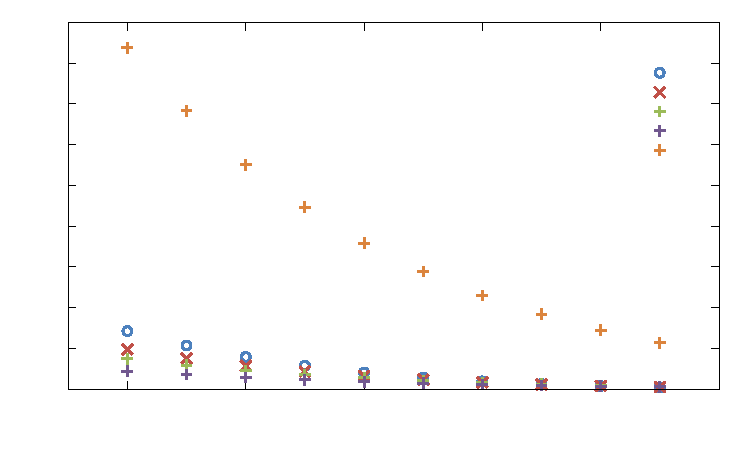
\includegraphics{GRAPH_distribution_of_magnification1}}%
    \gplfronttext
  \end{picture}%
\endgroup

					}\endgroup
		\end{minipage}
    	\begin{minipage}[c]{0.5\linewidth}
			\centering
				\begingroup\endlinechar=-1
					\resizebox{\textwidth}{!}{%
						% GNUPLOT: LaTeX picture with Postscript
\begingroup
  \makeatletter
  \providecommand\color[2][]{%
    \GenericError{(gnuplot) \space\space\space\@spaces}{%
      Package color not loaded in conjunction with
      terminal option `colourtext'%
    }{See the gnuplot documentation for explanation.%
    }{Either use 'blacktext' in gnuplot or load the package
      color.sty in LaTeX.}%
    \renewcommand\color[2][]{}%
  }%
  \providecommand\includegraphics[2][]{%
    \GenericError{(gnuplot) \space\space\space\@spaces}{%
      Package graphicx or graphics not loaded%
    }{See the gnuplot documentation for explanation.%
    }{The gnuplot epslatex terminal needs graphicx.sty or graphics.sty.}%
    \renewcommand\includegraphics[2][]{}%
  }%
  \providecommand\rotatebox[2]{#2}%
  \@ifundefined{ifGPcolor}{%
    \newif\ifGPcolor
    \GPcolortrue
  }{}%
  \@ifundefined{ifGPblacktext}{%
    \newif\ifGPblacktext
    \GPblacktexttrue
  }{}%
  % define a \g@addto@macro without @ in the name:
  \let\gplgaddtomacro\g@addto@macro
  % define empty templates for all commands taking text:
  \gdef\gplbacktext{}%
  \gdef\gplfronttext{}%
  \makeatother
  \ifGPblacktext
    % no textcolor at all
    \def\colorrgb#1{}%
    \def\colorgray#1{}%
  \else
    % gray or color?
    \ifGPcolor
      \def\colorrgb#1{\color[rgb]{#1}}%
      \def\colorgray#1{\color[gray]{#1}}%
      \expandafter\def\csname LTw\endcsname{\color{white}}%
      \expandafter\def\csname LTb\endcsname{\color{black}}%
      \expandafter\def\csname LTa\endcsname{\color{black}}%
      \expandafter\def\csname LT0\endcsname{\color[rgb]{1,0,0}}%
      \expandafter\def\csname LT1\endcsname{\color[rgb]{0,1,0}}%
      \expandafter\def\csname LT2\endcsname{\color[rgb]{0,0,1}}%
      \expandafter\def\csname LT3\endcsname{\color[rgb]{1,0,1}}%
      \expandafter\def\csname LT4\endcsname{\color[rgb]{0,1,1}}%
      \expandafter\def\csname LT5\endcsname{\color[rgb]{1,1,0}}%
      \expandafter\def\csname LT6\endcsname{\color[rgb]{0,0,0}}%
      \expandafter\def\csname LT7\endcsname{\color[rgb]{1,0.3,0}}%
      \expandafter\def\csname LT8\endcsname{\color[rgb]{0.5,0.5,0.5}}%
    \else
      % gray
      \def\colorrgb#1{\color{black}}%
      \def\colorgray#1{\color[gray]{#1}}%
      \expandafter\def\csname LTw\endcsname{\color{white}}%
      \expandafter\def\csname LTb\endcsname{\color{black}}%
      \expandafter\def\csname LTa\endcsname{\color{black}}%
      \expandafter\def\csname LT0\endcsname{\color{black}}%
      \expandafter\def\csname LT1\endcsname{\color{black}}%
      \expandafter\def\csname LT2\endcsname{\color{black}}%
      \expandafter\def\csname LT3\endcsname{\color{black}}%
      \expandafter\def\csname LT4\endcsname{\color{black}}%
      \expandafter\def\csname LT5\endcsname{\color{black}}%
      \expandafter\def\csname LT6\endcsname{\color{black}}%
      \expandafter\def\csname LT7\endcsname{\color{black}}%
      \expandafter\def\csname LT8\endcsname{\color{black}}%
    \fi
  \fi
  \setlength{\unitlength}{0.0500bp}%
  \begin{picture}(7200.00,4320.00)%
    \gplgaddtomacro\gplbacktext{%
      \put(747,595){\makebox(0,0)[r]{\strut{} 0}}%
      \put(747,1035){\makebox(0,0)[r]{\strut{} 0.2}}%
      \put(747,1475){\makebox(0,0)[r]{\strut{} 0.4}}%
      \put(747,1915){\makebox(0,0)[r]{\strut{} 0.6}}%
      \put(747,2355){\makebox(0,0)[r]{\strut{} 0.8}}%
      \put(747,2795){\makebox(0,0)[r]{\strut{} 1}}%
      \put(747,3235){\makebox(0,0)[r]{\strut{} 1.2}}%
      \put(747,3675){\makebox(0,0)[r]{\strut{} 1.4}}%
      \put(747,4115){\makebox(0,0)[r]{\strut{} 1.6}}%
      \put(1398,409){\makebox(0,0){\strut{} 10}}%
      \put(2497,409){\makebox(0,0){\strut{} 11}}%
      \put(3596,409){\makebox(0,0){\strut{} 12}}%
      \put(4695,409){\makebox(0,0){\strut{} 13}}%
      \put(5794,409){\makebox(0,0){\strut{} 14}}%
      \put(6893,409){\makebox(0,0){\strut{} 15}}%
      \csname LTb\endcsname%
      \put(144,2355){\rotatebox{-270}{\makebox(0,0){\strut{}Number of Galaxies}}}%
      \csname LTb\endcsname%
      \put(3871,130){\makebox(0,0){\strut{}Magnitude ($M$)}}%
      \put(3871,4022){\makebox(0,0){\strut{}}}%
    }%
    \gplgaddtomacro\gplfronttext{%
      \csname LTb\endcsname%
      \put(5987,3802){\makebox(0,0)[r]{\strut{}\SI{0.1e6}{\second}}}%
      \csname LTb\endcsname%
      \put(5987,3616){\makebox(0,0)[r]{\strut{}\SI{0.2e6}{\second}}}%
      \csname LTb\endcsname%
      \put(5987,3430){\makebox(0,0)[r]{\strut{}\SI{0.5e6}{\second}}}%
      \csname LTb\endcsname%
      \put(5987,3244){\makebox(0,0)[r]{\strut{}\SI{0.5e6}{\second}}}%
    }%
    \gplbacktext
    \put(0,0){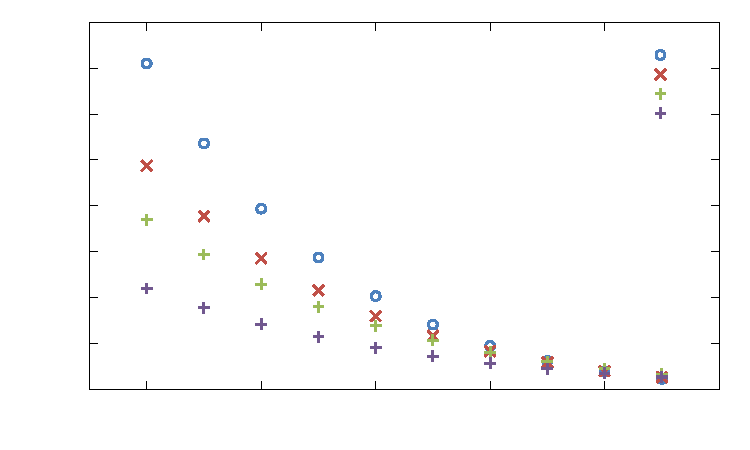
\includegraphics{GRAPH_distribution_of_magnification2}}%
    \gplfronttext
  \end{picture}%
\endgroup

					}\endgroup
		\end{minipage}
		\caption{Number of galaxies expected for different magnitudes, given set overall observing time (E-ELT 6--8.5).\label{fig:distribution_of_magnification1}}
	\end{figure}

	Even at the highest magnifications, few objects are expected at redshifts as high as 15, however at very small source angles, the magnification factor will be greater than 15 so there is the possibility of seeing very strongly lensed sources from even deeper redshifts. It is this potential for observing such high redshift objects that would make lensing a very valuable component of the strategy.

	There is a trade-off when using gravitational lenses between the ability to see much deeper due to the magnification and the fact that the viewing area is decreased due to obscuration by the lens and the increased size of the images. The lower the redshift of the lenses chosen, the more significant this problem is, pushing the optimum lens redshift towards a higher value again. As a result, the most useful way to integrate gravitational lensing into the strategy would be to use it as a supplement to the deep survey, to increase the number of objects observed at redshifts above 12 and to attempt to observe a few objects at extremely high redshift.
% subsection calculations_on_magnification (end)

	\subsubsection{Results and Planned Use of Gravitational Lensing} % (fold)
	\label{sub:results_and_planned_use_of_gravitational_lensing}
		It was decided that the most time efficient option was to choose known lenses since an additional survey would be required to locate new lenses. Combining the constraints set out in Section~\ref{sec:observational_gravitational_lensing}, an optimum lens redshift range of $0.5<z<0.7$ was chosen. A range of clusters lying within this redshift range were selected from the MACS catalogue. It was decided that lenses would be used in half of the deep field pointings in order to have a high chance of probing to the deepest redshifts while using the remaining fields without the obscuration caused by the lens. Table~\ref{tab:List_of_lenses_selected} lists the 5 chosen lenses with some of their key properties \cite{strong_lensing_analysis_MACS}. The locations of these lenses are well spread out, reducing cosmic variance.
		\begin{table}[htbp]
			\begin{center}
				\begin{tabular}{c||c|>{\centering\arraybackslash}m{2cm}|>{\centering\arraybackslash}m{2cm}|>{\centering\arraybackslash}m{1.6cm}|>{\centering\arraybackslash}m{3cm}}
	MACS Cluster 	& Redshift 	& $A$(J2000.0) (h m s) 	& $\Delta$(J2000.0) (${}^\circ$ ' '') & Mass ($10^{14} M_\odot$)	& Velocity dispersion (\si{\kilo\metre\per\second}) \\[0.4em]
	\hline\hline
	J0744.9+3927 	& 0.698 & 07:44:52.470 			& +39:27:27.34 	& $3.1\pm0.1$ 			& $1110_{-150}^{+130}$ \\[0.4em]
	J0025.4-1222 	& 0.584 & 00:25:29.381 			& -12:22:37.06 	& $2.42_{-0.13}^{+0.10}$ 	& $740_{-110}^{+90}$ \\[0.4em]
	J0257.1-2325 	& 0.505 & 02:57:09.151 			& -23:26:05.83 	& $3.35_{-0.10}^{+0.58}$ 	& $970_{-250}^{+200}$ \\[0.4em]
	J0647.7+7015 	& 0.591 & 06:47:50.469 			& +70:14:54.95 	& $2.07\pm0.1$ 			& $900_{-180}^{+120}$ \\[0.4em]
	J0911.2+1746 	& 0.505 & 09:11:11.277 			& +17:46:31.94 	& $2.07\pm0.1$ 			& $1150_{-340}^{+260}$
				\end{tabular}
			\end{center}
			\caption{List of lenses selected for the observing strategy.\label{tab:List_of_lenses_selected}}
		\end{table}

		It is worth noting that these lenses are all included in the HST Frontier Fields high magnification cluster candidate list, which lists massive clusters with highly efficient lensing properties increasing the likelihood of very high redshift sources being observed\cite{HST_strong_magnification}. The deeper the magnitude that is being observed, the longer it will take to observe the sources with a good signal to noise ratio. As a result, the depth probed will be balanced with observing time. Table~\ref{tab:observing_depths_and_number_of_lensed_objects} shows a range of observing depths and the number of lensed objects that would be seen at each.
		\begin{table}[htbp]
			\begin{center}
				\begin{tabular}{c||c|c|c|c|c|c|c|c}
		\multirow{2}{*}{MACS Cluster} & \multicolumn{2}{c|}{To Mag. 31.5}	&\multicolumn{2}{c|}{To Mag. 31} &\multicolumn{2}{c|}{To Mag. 30.5}	&\multicolumn{2}{c}{To Mag. 30}\\
					% MACS Cluster	&$10\!\le\! z\!\le\! 12$	&$12\!\le\! z\!\le\! 15$	&$10\!\le\! z\!\le\! 12$	&$12\!\le\! z\!\le\! 15$	&$10\!\le\! z\!\le\! 12$	&$12\!\le\! z\!\le\! 15$	&$10\!\le\! z\!\le\! 12$	&$12\!\le\! z\!\le\! 15$\\
					\cline{2-9}
						&A	&B	&A	&B	&A	&B	&A	&B\\
					\hline\hline
					J0025.4-1222	&10.6	&5	&3.1	&1.1	&5.9	&2.5	&2	&0.6\\
					J0257.1-2325	&33.9	&16.1	&10	&3.7	&19	&8	&6.3	&2\\
					J0647.7+7015	&23.1	&11	&6.8	&2.5	&13	&5.5	&4.3	&1.4\\
					J0744.9+3927	&49.3	&23.6	&14.6	&5.4	&27.7	&11.7	&9.1	&3\\
					J0911.2+1746	&66.9	&31.8	&19.8	&7.2	&37.5	&15.8	&12.4	&4
				\end{tabular}
			\end{center}
			\caption{Range of observing depths and number of lensed objects observed at redshift ranges 10-12 and 12-15 for each chosen lens. A columns are for $10\le z\le 12$ and B columns are for $12\le z\le 15$\label{tab:observing_depths_and_number_of_lensed_objects}}
		\end{table}

		These results indicate a significant increase in sources observed compared to the number expected without a lens. This is largely due to the rapid increase in the number of high redshift objects at dimmer magnitudes. The total number of extra galaxies expected from lensing is 183.9 at redshifts 10--12 and 87.5 at redshifts 12--15. This increase in the number of sources observed will give a much better sample of early galaxies, allowing tighter constraint to be placed on the epoch of reionization.

		While these calculations have a relatively large error due to uncertainty on the velocity dispersion, by far the dominant error affecting the number of extra galaxies seen results from cosmic variance. This error depends on the area which is being observed so the cosmic variance should be calculated for the area corresponding to each magnification factor for every lens and combined to give an overall value. The predictions group's program is not sufficiently complex to complete this calculation so using an average area (\SI{13180}{\arcsecond{}^2}) and velocity dispersion (\SI{974}{\kilo\metre\per\second}) from the 5 chosen lenses, the cosmic variance is, very roughly, found to be 64\%. This gives the total number of extra objects found to be $271\pm 174$, indicating that across the 5 lenses, a minimum of 97 extra galaxies should be observed, with at least 31 at redshifts greater than 12.

		Once candidates have been identified behind these clusters, spectroscopy will be used to confirm the source redshift and therefore the distance to the source. The mass and redshift of the lenses are known so equation~(\ref{eq:Einstein_radius}) can be used to find the Einstein angle. The magnification can then be calculated from equation~(\ref{eq:magnification_equation}). The flux from the images can be obtained from observations and can be used in conjunction with the magnification factor to calculate the intrinsic brightness of the source in bands redward of the drop from equation~(\ref{eq:mu_magnification}). Using model galaxy spectra, the flux in the band blueward of the drop can be estimated. This gives a lower limit on the neutral hydrogen fraction, since there must be at least enough to absorb the flux missing in the galaxy's spectrum\cite{lower_limit_H}.

		From these results, it is clear that that gravitational lensing will enable this strategy to better constrain the epoch of reionization by increasing the number of galaxies observed and by allowing surveys to probe significantly deeper redshifts.
	% subsection results_and_planned_use_of_gravitational_lensing (end)
